\documentclass[11pt]{article}
\usepackage[letterpaper,margin=0.85in]{geometry}
\usepackage[hidelinks]{hyperref}
\usepackage{enumitem}
\usepackage{titlesec}
\usepackage{tabularx}
\usepackage{graphicx}

\setlist[itemize]{leftmargin=1.2em,itemsep=3pt,topsep=3pt}
\titleformat{\section}{\large\bfseries}{}{0em}{}[\titlerule]

\newcommand{\entry}[4]{
  \noindent\begin{tabularx}{\textwidth}{@{}Xr@{}}
    \textbf{#1} & #2 \\
    \textit{#3} & \textit{#4}
  \end{tabularx}\vspace{2pt}
}

\begin{document}

\noindent\begin{minipage}[t]{0.76\textwidth}
\vspace{0pt}
{\LARGE \textbf{Piter Z. Garcia Bautista}}\\[4pt]
Rochester, NY \textbar\ +1 (646) 288-3300 \textbar\ \href{mailto:pzg8794@rit.edu}{pzg8794@rit.edu} \textbar\ \href{mailto:pitergarcia@rochester.edu}{pitergarcia@rochester.edu}\\
\href{https://linkedin.com/in/garciapiterz}{linkedin.com/in/garciapiterz} \textbar\
\href{https://github.com/pzg8794}{github.com/pzg8794} \textbar\
\href{https://garciapiterz.com}{garciapiterz.com}
\end{minipage}%
\hfill\begin{minipage}[t]{0.20\textwidth}
\vspace{0pt}
\raggedleft
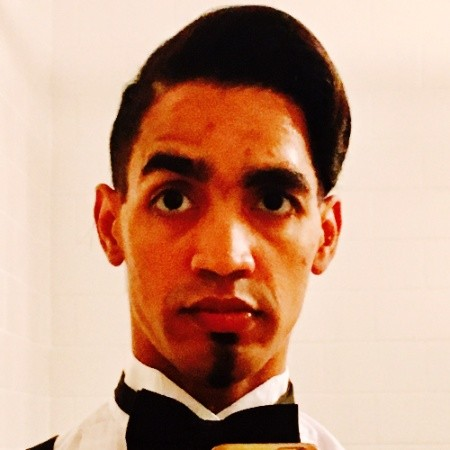
\includegraphics[width=\linewidth]{profile_pic}
\end{minipage}
\vspace{6pt}

\section{Research Profile}
NSF Robert Noyce Scholar and graduate researcher working at the intersection of adaptive machine learning, fairness-aware AI, and high-stakes decision support in dynamic, noisy operational environments. Background spans reproducible evaluation systems for sequential decision-making, contextual bandit methods, and fairness-aware ML applied to clinical and biological data. Current Graduate Assistant work (Quantum and AI Research, RIT) emphasizes reliability under shifting operational conditions and rigorous evaluation methodology. Computational biology training in RNA structure prediction (BIO614) and RNA-seq differential expression analysis (BIO550) complements this with practical experience in biological data pipelines. CS teaching and education research (NSF Noyce Scholar, UofR Warner School) adds a data-driven research thread on AI-informed adaptive learning design for neurodivergent students. Motivated to apply this adaptive, uncertainty-aware ML expertise to maritime environmental monitoring problems: reliable inference under noisy sensor streams, constrained communication, and non-stationary environmental dynamics.

\section{Research Interests}
Adaptive ML for non-stationary sensor-driven environments; contextual and sequential decision-making under uncertainty; fairness-aware and trustworthy AI for high-stakes monitoring and decision support; reproducible evaluation systems for distributed and constrained settings; computational biology and data-driven approaches to equitable education.

\section{Education}

\entry{Rochester Institute of Technology}{Expected Aug 2026}{Master of Science, Data Science --- GPA 3.9}{Rochester, NY}
\begin{itemize}
  \item Concentration: Bioinformatics \& Artificial Intelligence.
  \item Relevant coursework: Foundations of Data Science (DSCI-633), Software Engineering for Data Science (DSCI-644), Applied Data Science I (DSCI-601), Bioinformatics Algorithms (BIOL-630), Data-Driven Knowledge Discovery (ISTE-780).
\end{itemize}

\entry{University of Rochester, Warner School of Education}{Expected Aug 2026}{Master of Science track, Teaching Computer Science K--12 --- GPA 4.0}{Rochester, NY}
\begin{itemize}
  \item NSF Robert Noyce Teacher Scholarship Program (\$30,000 full funding).
  \item Advanced Certificate in Leadership in Disability and Inclusive Practices.
\end{itemize}

\entry{Rochester Institute of Technology}{2015}{Master of Science, Computer Science --- GPA 3.2}{Rochester, NY}
\begin{itemize}
  \item Concentrations: Computer Graphics, Artificial Intelligence, Big Data Analytics.
\end{itemize}

\entry{Farmingdale State College}{2012}{Bachelor of Science, Computer Engineering Technology --- GPA 3.3}{Farmingdale, NY}
\begin{itemize}
  \item Dual degree: Electrical Engineering \& Computer Engineering Technology.
  \item Honors: CSTEP Award \& Merit, Dual BS Scholarship.
\end{itemize}

\section{Research and Professional Experience}

\entry{Rochester Institute of Technology, Software Engineering Department}{Fall 2025 -- Present}{Graduate Assistant, Quantum and AI Research}{Rochester, NY}
\begin{itemize}
  \item Build reproducible ML evaluation pipelines across local, Colab, and GCP environments for bandit and routing experiments under stochastic and adversarial settings.
  \item Develop contextual and sequential decision-making systems with structured logging, multi-run reproducibility, and statistical validation.
  \item Produce manuscript-ready technical analyses covering reliability-first evaluation methodology and structured experimental design.
\end{itemize}

\entry{University of Rochester, Warner School of Education}{Sep 2024 -- Present}{CS Teacher Candidate \& Education Research (NSF Noyce Scholar)}{Rochester, NY}
\begin{itemize}
  \item Deliver K--12 computer science instruction in active public school placement as part of the NSF Robert Noyce Scholar program, including computational thinking, inclusive pedagogy, and NYS learning standards.
  \item Conduct applied education research on AI-informed and data-driven approaches to improve learning outcomes for neurodivergent students, applying Universal Design for Learning (UDL) and evidence-based adaptive strategies.
  \item Produce lesson artifacts and instructional analyses documenting the intersection of AI, inclusive education, and evidence-based CS pedagogy.
\end{itemize}

\entry{Rochester Institute of Technology}{2024 -- 2025}{Principal Investigator, Equitable Bioinformatics Research (ISTE-780)}{Rochester, NY}
\begin{itemize}
  \item Applied systematic fairness analysis to RNA secondary structure prediction pipelines; demonstrated statistical significance ($p < 0.01$) in bias detection across algorithmic variants using SHAP and disparity-impact analysis.
  \item Implemented reproducible evaluation codebase (900+ lines) with automated metric reporting and statistical testing.
\end{itemize}

\entry{Rochester Institute of Technology}{2025 -- 2026}{Computational Biology Research (BIO614 and BIO550)}{Rochester, NY}
\begin{itemize}
  \item Led formal computational analysis in BIO614: advanced RNA secondary structure prediction with thermodynamic MFE enhancements; produced \textit{BIO614-FinalProjectProposal} (Overleaf manuscript).
  \item Conducted reproducible bulk RNA-seq differential-expression analysis (BIO550): DESeq2 pipeline with QC validation, alignment review, and pathway-level biological interpretation of nociceptor gene expression.
\end{itemize}

\entry{VEDADATA Inc.}{Sep 2022 -- Aug 2024}{Data Solutions Engineer}{New York, NY}
\begin{itemize}
  \item Designed scalable Python data pipelines for ingestion, validation, statistical diagnostics, and analytics operations.
  \item Strengthened production reliability through structured quality checks and anomaly detection.
\end{itemize}

\entry{VIOME Inc.}{Jan 2021 -- Sep 2022}{AI Data Solutions Engineer}{New York, NY}
\begin{itemize}
  \item Developed healthcare AI workflows including deep learning feature engineering, model experimentation, and evaluation.
  \item Built preprocessing pipelines for microbiome sequencing data, including normalization, QC filtering, and feature extraction.
\end{itemize}

\section{Selected Technical Writing}
\begin{itemize}
  \item \textit{Big Data Medical Diagnosis: A Multi-Method Approach} (RIT M.S.\ Computer Science graduate research, 2015) --- ensemble and deep learning methods for clinical classification on high-dimensional biomedical data.
  \item \textit{Predicting Hospital Readmission Rates: A Multi-Method ML Analysis} (DSCI-633 Project Report, 2025) --- ensemble and regularized regression methods for clinical risk stratification under distribution shift.
  \item \textit{BIO614-FinalProjectProposal} (Overleaf manuscript, 2026) --- RNA secondary structure prediction with thermodynamic deep learning enhancements, reproducible benchmarking, and biological interpretation.
  \item \textit{Equitable Bioinformatics: Enhancing Diagnostic Decision-Making through RNA and Biomarker Data} (ISTE-780 Project Report, 2025) --- fairness-aware ML for genomic diagnostic algorithms with SHAP-based bias detection and statistical significance testing.
  \item \textit{Differential Gene Expression in Murine DRG Neurons Following Sciatic Nerve Injury: An NGS Reanalysis} (BIOL550 Computational Biology Project, 2026) --- reproducible bulk RNA-seq pipeline using DESeq2, QC validation, and pathway-level biological interpretation of nociceptor gene expression.
  \item \textit{Fairness-Aware Bandits for Clinical Decision Systems} (DSCI-601 Project Proposal, 2025) --- bandit learning with equity constraints applied to high-stakes clinical diagnostic decision-making, addressing demographic disparity and sequential recommendation for patient triage and risk stratification.
\end{itemize}

\section{Awards \& Recognition}
\begin{itemize}
  \item NSF Robert Noyce Teacher Scholarship (2024--2026) --- full funding for M.S. in Teaching Computer Science K--12.
  \item MS International Scholarship (2012--2015) --- MESCYT \& RIT, awarded for academic excellence.
  \item Honorable Mention Technology Award (2012) --- NYS STEP/CSTEP, 2nd place capstone project.
  \item IEEE Alumni Member (2009--Present) --- Member No. 90613000.
\end{itemize}

\section{Technical Competencies}
\textbf{Programming:} Python, R, Java, C++, C\#, MATLAB, SQL, JavaScript, Bash\\
\textbf{Machine Learning:} PyTorch, TensorFlow, scikit-learn, XGBoost, fairness-aware ML, contextual bandit workflows, sequential decision-making\\
\textbf{Data \& Analysis:} pandas, NumPy, SciPy, SHAP analysis, statistical testing, reproducible benchmarking\\
\textbf{Infrastructure:} AWS, GCP, Docker, Git/GitHub, Linux, LaTeX

\section{Selected Fit for NTNU AI-Enabled Maritime Systems Position}
\begin{itemize}
  \item Strong fit for adaptive maritime monitoring research through experience with dynamic decision workflows, reliability analysis, and constrained-system evaluation.
  \item Demonstrated reproducibility discipline for multi-run experimental design, statistical validation, and transparent reporting.
  \item Interdisciplinary AI background spanning method development, applied data systems, and high-stakes deployment contexts.
\end{itemize}

\end{document}
